% !TEX TS-program = XeLaTeX
% use the following command:
% all document files must be coded in UTF-8
\documentclass[portuguese]{textolivre}
% build HTML with: make4ht -e build.lua -c textolivre.cfg -x -u article "fn-in,svg,pic-align"

\journalname{Texto Livre}
\thevolume{18}
%\thenumber{1} % old template
\theyear{2025}
\receiveddate{\DTMdisplaydate{2025}{3}{27}{-1}} % YYYY MM DD
\accepteddate{\DTMdisplaydate{2025}{6}{9}{-1}}
\publisheddate{\DTMdisplaydate{2025}{10}{24}{-1}}
\corrauthor{Laura Paola Ferreira}
\articledoi{10.1590/1983-3652.2025.58366}
%\articleid{NNNN} % if the article ID is not the last 5 numbers of its DOI, provide it using \articleid{} commmand 
% list of available sesscions in the journal: articles, dossier, reports, essays, reviews, interviews, editorial
\articlesessionname{articles}
\runningauthor{Ferreira, César e Rossoni} 
%\editorname{Leonardo Araújo} % old template
\sectioneditorname{Daniervelin Pereira}
\layouteditorname{Leonado Araújo}

\title{A abordagem triangular no ensino de arte: uma proposta educacional integrada}
\othertitle{The triangular approach in art education: an integrated educational proposal}
% if there is a third language title, add here:
%\othertitle{Artikelvorlage zur Einreichung beim Texto Livre Journal}

\author[1]{Laura Paola Ferreira~\orcid{0000-0002-9397-5055}\thanks{Email: \href{mailto:laura.ferreira@uemg.br}{laura.ferreira@uemg.br}}}
\author[1]{Danilo Rodrigues Zinatelli César~\orcid{0000-0002-6640-1136}\thanks{Email: \href{mailto:danilorcesar@gmail.com}{danilorcesar@gmail.com}}}
\author[2]{Eloiza Mara de Paula Rossoni~\orcid{0000-0001-9933-9570}\thanks{Email: \href{mailto:elorossoniartista@gmail.com}{elorossoniartista@gmail.com}}}
\affil[1]{Universidade Estadual de Minas Gerais, Pedagogia, Departamento de
Educação, Ibirité, MG, Brasil.}
\affil[2]{Universidade Federal de Minas Gerais, Belo Horizonte, MG, Brasil.}

\addbibresource{article.bib}
% use biber instead of bibtex
% $ biber article

% used to create dummy text for the template file
\definecolor{dark-gray}{gray}{0.35} % color used to display dummy texts
\usepackage{lipsum}
\SetLipsumParListSurrounders{\colorlet{oldcolor}{.}\color{dark-gray}}{\color{oldcolor}}

% used here only to provide the XeLaTeX and BibTeX logos
\usepackage{hologo}

% if you use multirows in a table, include the multirow package
\usepackage{multirow}

% provides sidewaysfigure environment
\usepackage{rotating}

% CUSTOM EPIGRAPH - BEGIN 
%%% https://tex.stackexchange.com/questions/193178/specific-epigraph-style
\usepackage{epigraph}
\renewcommand\textflush{flushright}
\makeatletter
\newlength\epitextskip
\pretocmd{\@epitext}{\em}{}{}
\apptocmd{\@epitext}{\em}{}{}
\patchcmd{\epigraph}{\@epitext{#1}\\}{\@epitext{#1}\\[\epitextskip]}{}{}
\makeatother
\setlength\epigraphrule{0pt}
\setlength\epitextskip{0.5ex}
\setlength\epigraphwidth{.7\textwidth}
% CUSTOM EPIGRAPH - END

% to use IPA symbols in unicode add
%\usepackage{fontspec}
%\newfontfamily\ipafont{CMU Serif}
%\newcommand{\ipa}[1]{{\ipafont #1}}
% and in the text you may use the \ipa{...} command passing the symbols in unicode

% LANGUAGE - BEGIN
% ARABIC
% for languages that use special fonts, you must provide the typeface that will be used
% \setotherlanguage{arabic}
% \newfontfamily\arabicfont[Script=Arabic]{Amiri}
% \newfontfamily\arabicfontsf[Script=Arabic]{Amiri}
% \newfontfamily\arabicfonttt[Script=Arabic]{Amiri}
%
% in the article, to add arabic text use: \textlang{arabic}{ ... }
%
% RUSSIAN
% for russian text we also need to define fonts with support for Cyrillic script
% \usepackage{fontspec}
% \setotherlanguage{russian}
% \newfontfamily\cyrillicfont{Times New Roman}
% \newfontfamily\cyrillicfontsf{Times New Roman}[Script=Cyrillic]
% \newfontfamily\cyrillicfonttt{Times New Roman}[Script=Cyrillic]
%
% in the text use \begin{russian} ... \end{russian}
% LANGUAGE - END

% EMOJIS - BEGIN
% to use emoticons in your manuscript
% https://stackoverflow.com/questions/190145/how-to-insert-emoticons-in-latex/57076064
% using font Symbola, which has full support
% the font may be downloaded at:
% https://dn-works.com/ufas/
% add to preamble:
% \newfontfamily\Symbola{Symbola}
% in the text use:
% {\Symbola }
% EMOJIS - END

% LABEL REFERENCE TO DESCRIPTIVE LIST - BEGIN
% reference itens in a descriptive list using their labels instead of numbers
% insert the code below in the preambule:
%\makeatletter
%\let\orgdescriptionlabel\descriptionlabel
%\renewcommand*{\descriptionlabel}[1]{%
%  \let\orglabel\label
%  \let\label\@gobble
%  \phantomsection
%  \edef\@currentlabel{#1\unskip}%
%  \let\label\orglabel
%  \orgdescriptionlabel{#1}%
%}
%\makeatother
%
% in your document, use as illustraded here:
%\begin{description}
%  \item[first\label{itm1}] this is only an example;
%  % ...  add more items
%\end{description}
% LABEL REFERENCE TO DESCRIPTIVE LIST - END


% add line numbers for submission
%\usepackage{lineno}
%\linenumbers

\begin{document}
\maketitle

\begin{polyabstract}
\begin{abstract}
Este artigo investiga a aplicação da abordagem triangular no ensino de arte, destacando seus fundamentos e benefícios educacionais. A metodologia triangular, desenvolvida por Ana Mae Barbosa, integra três eixos – apreciação, contextualização e criação – para enriquecer o processo de aprendizagem e promover o desenvolvimento crítico e estético dos alunos. Adotando uma metodologia qualitativa, o estudo baseia-se em uma revisão bibliográfica abrangente de obras teóricas e estudos de caso que exemplificam a prática da abordagem em diferentes contextos educacionais. A análise de conteúdo das fontes coletadas revela que a apreciação permite que os estudantes interpretem criticamente as obras, a contextualização os conecta aos aspectos históricos e culturais, e a criação incentiva a expressão pessoal e o domínio técnico. Além disso, a integração de tecnologias digitais, como recursos multimídia e plataformas de compartilhamento, potencializa a interatividade e a acessibilidade das práticas pedagógicas, enriquecendo a experiência educacional. Os resultados indicam que a abordagem triangular, aliada ao uso de tecnologias, proporciona um modelo de educação artística mais significativo, preparando os alunos para serem cidadãos críticos, engajados em sua realidade cultural. Em conclusão, a abordagem triangular destaca-se como um recurso pedagógico relevante e eficaz no ensino de arte.

\keywords{Educação artística \sep Práticas pedagógicas inovadoras \sep Análise crítica da arte \sep Contextualização cultural \sep Tecnologia educacional}
\end{abstract}

\begin{english}
\begin{abstract}
This article investigates the application of the triangular approach in art education, highlighting its foundations and educational benefits. The triangular methodology, developed by Ana Mae Barbosa, integrates three axes — appreciation, contextualization, and creation — to enrich the learning process and promote students' critical and aesthetic development. Adopting a qualitative methodology, the study is based on a comprehensive bibliographic review of theoretical works and case studies that exemplify the practice of the approach in different educational contexts. The content analysis of the collected sources reveals that appreciation allows students to critically interpret artworks, contextualization connects them to historical and cultural aspects, and creation encourages personal expression and technical mastery. Additionally, the integration of digital technologies, such as multimedia resources and sharing platforms, enhances the interactivity and accessibility of pedagogical practices, enriching the educational experience. The results indicate that the triangular approach, combined with the use of technologies, provides a more meaningful art education, preparing students to be critical citizens engaged in their cultural reality. In conclusion, the triangular approach stands out as a relevant and effective pedagogical resource in art education.

\keywords{Art education \sep Innovative pedagogical practices \sep Critical art analysis \sep Cultural contextualization \sep Educational technology}
\end{abstract}
\end{english}
% if there is another abstract, insert it here using the same scheme
\end{polyabstract}

\section{Introdução}\label{sec-intro}
O ensino em arte tem um papel central no desenvolvimento de competências críticas, estéticas e culturais, que podem proporcionar aos estudantes recursos para interpretar o mundo e a si mesmos de forma mais abrangente. No contexto educacional brasileiro, a abordagem triangular proposta por Ana Mae Barbosa, de certa forma, revolucionou o ensino de artes ao introduzir uma metodologia que integra três eixos fundamentais: apreciação, contextualização e criação. \textcite{barbosa2008educacao} defende que essa metodologia oferece uma “prática educacional crítica e libertadora”, de modo a estimular os alunos a interagirem com a arte de maneira completa e significativa. Para Barbosa, o ensino de arte precisa ser uma prática que não apenas ensine técnicas, mas que promova o entendimento cultural e o desenvolvimento de uma “visão crítica sobre o mundo” \cite{barbosa2010arte}.

Nesse sentido, a metodologia triangular tem como um de seus focos o desenvolvimento da capacidade de apreciação crítica da arte, que envolve a análise e a interpretação de obras de forma aprofundada. De acordo com \textcite{barbosa2010arte}, “apreciar é interpretar e se deixar afetar pela obra de arte”, uma prática que incentiva a reflexão e a construção de significado a partir da experiência estética. Isso permite que os estudantes se envolvam com a obra de arte em níveis pessoais e críticos, fomentando uma relação significativa com a produção artística.

O segundo eixo da abordagem triangular, a contextualização, propõe que a arte seja entendida em seu contexto histórico, social e cultural. \textcite{barbosa2008educacao} argumenta que “a arte não pode ser ensinada em isolamento”, pois é parte integrante das dinâmicas sociais e culturais. Assim, o ensino de arte deve promover uma compreensão das obras que considere seus aspectos históricos e culturais, conectando os estudantes ao tempo e ao espaço em que essas produções foram concebidas. Esse eixo fomenta a visão crítica informada, uma vez que possibilita uma análise da arte que leva em conta fatores externos e significativos para a interpretação do seu conteúdo.

O terceiro eixo, criação, incentiva os estudantes a desenvolverem suas próprias expressões artísticas, utilizando o conhecimento adquirido nos processos de apreciação e contextualização. Para \textcite{barbosa2009arte}, a criação é o “momento em que o estudante se coloca como produtor cultural”, construindo seu repertório técnico e pessoal. Esse processo de criação fortalece o desenvolvimento de habilidades técnicas e permite que os estudantes explorem suas identidades e perspectivas, consolidando uma prática educacional que valoriza tanto a expressão individual quanto a autonomia criativa.

É importante salientar que, na atualidade, no “mundo conectado ao digital”, a inclusão da tecnologia no ensino de arte é uma tendência crescente que pode auxiliar a abordagem triangular. Recursos digitais, como \textit{softwares} de \textit{design}, aplicativos de edição e plataformas de compartilhamento de arte, ampliam as possibilidades de criação e expressão artística. Segundo \textcite{dewey1934art}, a experiência estética se enriquece quando os alunos têm acesso a diferentes meios de expressão, tornando-se ativos na construção de seu próprio conhecimento. Além disso, a tecnologia facilita a apreciação e a contextualização da arte, permitindo que os alunos explorem obras de forma interativa e conectada ao seu contexto histórico e cultural \cite{freire1996aautonomia}.

A adoção da abordagem triangular no ensino de arte é, portanto, uma estratégia pedagógica que promove a formação integral dos alunos, ao equilibrar teoria e prática e estimular uma visão crítica da arte e da cultura. Segundo \textcite{lopes2013metodologias}, essa abordagem “potencializa o aprendizado ao integrar aspectos críticos e criativos”, um processo que reflete os princípios de uma educação mais completa e inclusiva. A importância da abordagem triangular se destaca ainda mais quando se considera a necessidade de um modelo de educação que prepare os estudantes para a compreensão mais ampla e sensível do mundo ao seu redor; e a combinação da abordagem triangular com a tecnologia pode resultar em uma experiência educacional mais abrangente, com vistas a estimular a curiosidade, a criatividade e o pensamento crítico dos estudantes. Museus e galerias, por exemplo, têm adotado exposições virtuais e visitas guiadas \textit{online}, proporcionando aos alunos a oportunidade de interagir com obras de arte de maneira significativa e contextualizada \cite{barbosa2010arte}. A educação artística contemporânea, ao integrar tecnologia e metodologia inovadora, pode ser um catalisador para ajudar a formar cidadãos plenos.

Com base nesses fundamentos, o presente artigo busca investigar o desenvolvimento da abordagem triangular em contextos educacionais diversos e analisar os impactos dessa metodologia no desenvolvimento crítico e estético dos alunos. A pesquisa baseia-se em uma revisão de literatura que engloba estudos teóricos e práticos, oferecendo uma análise detalhada dos benefícios e desafios do uso dessa abordagem no ensino de arte. Além disso, pretende-se explorar casos práticos em instituições educacionais, com ênfase nos resultados observados.

Assim, por meio desta investigação, espera-se oferecer subsídios teóricos e práticos que possam auxiliar educadores na adoção de estratégias pedagógicas que integrem a abordagem triangular, tornando as aulas de arte em momentos de aprendizado transformador e enriquecedor. Portanto, a análise das implicações da abordagem triangular no ensino de arte se revela não apenas pertinente, mas essencial para a construção de um modelo de educação que respeite e valorize a diversidade cultural e que favoreça o desenvolvimento integral dos estudantes no atual cenário educacional.

\section{Revisão de literatura}\label{sec-normas}
A educação artística, como campo de estudo e prática pedagógica, tem se transformado ao longo das últimas décadas, refletindo mudanças sociais, culturais e teóricas. Nesse contexto, a abordagem triangular, proposta por Ana Mae Barbosa, destaca-se como inovadora. Esta seção trata, pois, de alguns itens da literatura sobre o Ensino de Arte e a Abordagem Triangular, buscando compreender suas bases teóricas e a relevância de sua aplicação no ensino de arte.

\subsection{A educação artística e suas abordagens}
Historicamente, a educação artística tem sido marcada por diversas abordagens que vão desde a simples instrução técnica até práticas mais reflexivas e críticas. A abordagem tradicional, por exemplo, que enfatiza a reprodução técnica de obras de arte, foi amplamente criticada por limitar a experiência estética dos alunos e não promover uma compreensão mais ampla da arte \cite{bourdieu1996distincao}. Nesse sentido, autores como \textcite{freire1996boprimido} defendem a educação que promova a reflexão crítica e a autonomia do estudante e, nesse contexto, propõem que a arte seja vista como um meio de expressão e transformação social.

Com a introdução de novas perspectivas, o ensino de arte começou a incorporar abordagens que favorecem a reflexão e o diálogo. Nesse contexto, a tecnologia aparece como um recurso valioso que pode facilitar essa contextualização. Recursos digitais permitem que os alunos explorem a história da arte e suas conexões culturais de maneiras interativas e envolventes, enriquecendo sua compreensão e apreciando a diversidade artística. A ideia de que a arte deve ser contextualizada, levando em conta as realidades socioculturais dos alunos, ganha destaque em pesquisas recentes \cite{hernandez2000educacao}. Segundo essa visão, a prática artística não deve ser dissociada do contexto histórico e cultural em que está inserida, permitindo que os alunos desenvolvam compreensão crítica e informada das obras e movimentos artísticos. Essa conexão entre arte e contexto social é reforçada por \textcite{lopes2013metodologias}, que argumentam que, na educação artística, deve haver diálogo entre diferentes culturas e experiências, que promova a formação que respeite a diversidade.

\subsection{A abordagem triangular de Ana Mae Barbosa}
A Abordagem Triangular, por sua vez, propõe um modelo de ensino que visa à aprendizagem significativa. Segundo \textcite{barbosa2010arte}, essa abordagem visa não apenas o desenvolvimento técnico, mas também o aprimoramento da sensibilidade estética e crítica dos alunos. Ao articular os eixos, a metodologia triangular promove um espaço de aprendizagem em que a arte é compreendida de maneira integrada, levando em consideração as influências culturais e sociais que a moldam.

\textcite{barbosa2010arte} salienta que a apreciação crítica é fundamental para que os alunos possam desenvolver um olhar reflexivo sobre a arte, reconhecendo suas diversas significações e contextos. Isso se dá de modo processual, em que os estudantes passam de meros espectadores a participantes ativos na construção de significados.

O pilar da contextualização, nesse contexto, busca conectar os alunos às narrativas históricas, sociais e culturais que permeiam as obras de arte. \textcite{hernandez2000educacao} ressalta que a contextualização é essencial para que os alunos compreendam a arte como um fenômeno social, influenciado por fatores como classe, gênero e etnia. Ao integrar a contextualização ao ensino, os educadores oferecem aos alunos recursos para que possam relacionar a arte com suas próprias experiências e realidades. Essa conexão serve para alavancar o desenvolvimento da visão crítica, uma vez que os alunos podem identificar como a arte reflete e impacta suas vidas e seus contextos sociais.

Na sequência, a criação é o eixo que incentiva a expressão pessoal e a experimentação artística. \textcite{barbosa2010arte} argumenta que a criação deve ser estimulada em um ambiente de liberdade e acolhimento, onde os alunos se sintam seguros para explorar suas próprias ideias e emoções. Essa liberdade criativa é crucial para o desenvolvimento da autonomia e da identidade dos estudantes, permitindo que eles se expressem de maneira autêntica. \textcite{lopes2013metodologias} corroboram essa ideia, ressaltando que a criação artística, além de ser uma habilidade técnica, é também um processo de autoconhecimento e descoberta.

\subsection{Práticas e eficácia da abordagem triangular}

Diversos estudos têm demonstrado a eficácia da abordagem triangular na promoção de um modelo de educação artística mais abrangente. Entre eles, \textcite{lopes2013metodologias} conduziram um estudo de caso em uma escola pública, onde a aplicação da metodologia triangular resultou em um aumento significativo do engajamento dos alunos nas atividades artísticas. Os autores observaram que, ao serem estimulados a apreciar e contextualizar as obras, os estudantes desenvolveram capacidade crítica e compreensão mais profunda da arte.

Além disso, a abordagem triangular tem sido utilizada com sucesso em contextos fora da sala de aula, como em museus e centros culturais. No Museu de Arte Contemporânea da Universidade de São Paulo (MAC-USP), por exemplo, essa abordagem foi aplicada em oficinas que envolveram os três eixos: apreciação, contextualização e criação de obras de arte. \textcite{barbosa2010arte} relata que essas oficinas enriqueceram a experiência dos alunos, além de promover o diálogo significativo entre arte e sociedade. Desse modo, entende-se que o envolvimento dos estudantes em experiências práticas de criação artística, tanto dentro quanto fora da sala de aula, contribui para uma relação mais profunda com a arte e a cultura.

\textcite{ferreira2015praticas} identificaram que a implementação da abordagem triangular em diferentes contextos educacionais pode aprimorar a percepção estética dos alunos, como também os capacitar a se tornarem críticos conscientes, reflexivos. Esses efeitos transcendem o âmbito artístico, pois podem contribuir no desenvolvimento de habilidades transversais, como pensamento analítico, comunicação e argumentação.

\subsection{BNCC e a abordagem triangular}
Apesar de este trabalho não ter como foco correlacionar a Abordagem Triangular de Ana Mae Barbosa com a Base Nacional Curricular Comum (BNCC) \cite{brasil2018bncc}, entende-se ser importante apresentar uma síntese dessa correlação. Salienta-se que a abordagem de Barbosa encontra ressonância direta nas competências e habilidades previstas pela BNCC para o ensino de Arte. Quando a BNCC propõe que os alunos "reconheçam e apreciem manifestações artísticas" (Competência Específica 1 - CE1 - Valorização artística), isso se concretiza por meio da apreciação crítica de obras, pela qual os estudantes desenvolvem habilidades de análise formal e interpretação (EF69AR04 – Análise de obras). Da mesma forma, a exigência da BNCC por contextualização histórica (CE4 - Arte como produção cultural) é atendida quando os alunos investigam as condições sociais e culturais que influenciaram movimentos artísticos (EF69AR06 – Relação história-arte), como ao relacionarem o modernismo brasileiro com o projeto de identidade nacional da década de 1920. Esses dois primeiros eixos preparam o contexto para a produção prática que, na BNCC, aparece como “experimentação de linguagens” (CE2 – Experimentação), permitindo que os estudantes criem trabalhos autorais a partir dos repertórios estudados (EF15AR02 – Fazer artístico).

A correlação entre as duas propostas se mostra especialmente evidente no desenvolvimento do pensamento crítico (Competência Geral 4 – Pensamento crítico) e da autonomia criativa (Competência Geral 2 – Autonomia criativa). Enquanto a Abordagem Triangular oferece a estrutura metodológica para articular olhar, compreensão e fazer artístico, a BNCC estabelece as competências necessárias para que essa tríade se traduza em aprendizagens significativas. Por exemplo, ao trabalhar com grafite urbano, os alunos podem apreciar obras de artistas como Banksy (EF69AR04), pesquisar seu surgimento como forma de protesto político (EF69AR06) e produzir intervenções visuais na escola (EF15AR02) – atividade que integra ainda a Competência Geral 5 (Cultura digital) quando documentam o processo em formatos multimídia.

Essa integração entre a Abordagem Triangular e a BNCC resulta em um modelo de ensino de Arte mais coerente e transformador, no qual o conhecimento artístico não se limita à técnica, mas forma cidadãos capazes de ler criticamente o mundo e nele intervir criativamente (Competência Geral 3 – Fruição artística). Tanto Barbosa quanto a Base entendem a arte como linguagem carregada de significado cultural, e sua conjugação na prática pedagógica permite que os estudantes desenvolvam simultaneamente sensibilidade estética e consciência social – dois pilares fundamentais para a educação contemporânea que dialogam com as Competências Gerais 8 e 9 da BNCC, relativas à empatia e responsabilidade social.

\subsection{Considerações finais da revisão}
A literatura evidencia a eficácia da abordagem triangular como recurso pedagógico transformador no ensino de arte. Seus três eixos permitem aos educadores criar experiências que formam indivíduos mais conscientes e engajados. Ao integrar apreciação, contextualização e criação, a metodologia amplia a experiência estética dos alunos e os capacita a interpretar e agir criticamente em um mundo em constante mudança.

Assim, a literatura aponta a urgência de repensar as práticas educacionais de ensino de arte, substituindo abordagens tradicionais por métodos mais críticos e integrativos, em sintonia com a formação cidadã. Nesse contexto, a metodologia triangular destaca-se como essencial para uma educação artística alinhada às demandas do século 21. Salienta-se que a incorporação da tecnologia pode ainda potencializar sua aplicação, ampliando interações e relevância.

\section{Metodologia}\label{sec-conduta}
Este estudo adota uma abordagem qualitativa, fundamentada em uma revisão bibliográfica e na análise de conteúdo, com o intuito de explorar os impactos e as aplicações da abordagem triangular no ensino de arte. A pesquisa qualitativa é especialmente adequada para a investigação do ensino artístico, uma vez que permite a compreensão mais profunda das práticas educacionais e dos processos de aprendizagem que envolvem os eixos apreciação, contextualização e criação (Minayo, 2010). Além disso, a pesquisa qualitativa oferece um espaço para dar voz aos participantes, permitindo que suas experiências e percepções sejam consideradas na análise.

A revisão da literatura foi conduzida a partir da seleção e análise de livros, artigos científicos e documentos acadêmicos que discutem a abordagem triangular, focando em autores como Ana Mae Barbosa, que é uma referência no desenvolvimento dessa metodologia. O levantamento bibliográfico buscou identificar as bases teóricas e as práticas pedagógicas associadas à abordagem triangular, bem como os resultados de estudos anteriores que analisaram a eficácia dessa metodologia em contextos educacionais variados \cite{barbosa2010arte,hernandez2000educacao}. A análise bibliográfica possibilitou um entendimento aprofundado dos fundamentos e objetivos da abordagem triangular, além de evidenciar as variações em sua aplicação em diferentes realidades escolares.

A análise de conteúdo dos materiais coletados se deu em seguida. Essa, segundo \textcite{bardin2011analise}, é uma técnica que permite interpretar mensagens de maneira objetiva e sistemática, particularmente útil para identificar temas, categorias e padrões recorrentes nas práticas educacionais documentadas. Essa técnica foi utilizada para investigar como os três eixos são aplicados em sala de aula, visando compreender o impacto de cada um deles na formação estética e crítica dos alunos. Durante o processo de análise, foi dada atenção especial às práticas que evidenciam o potencial da abordagem triangular em fomentar o desenvolvimento crítico e a autonomia criativa dos estudantes.

Outro elemento relevante no processo metodológico foi a análise de estudos de caso que exemplificam a prática da abordagem triangular em diferentes contextos educacionais, incluindo escolas públicas, privadas e instituições de ensino superior. Essa etapa permitiu observar as particularidades e os desafios da implementação da abordagem triangular em diferentes níveis de ensino e com diferentes faixas etárias. Estudos de casos de instituições como o Museu de Arte Contemporânea da Universidade de São Paulo (MAC-USP) demonstram a eficácia da metodologia triangular quando aplicada em espaços culturais, proporcionando aos alunos uma vivência prática e contextualizada da arte \cite{barbosa2010arte,lopes2013metodologias}.

A metodologia aplicada neste estudo permitiu uma compreensão detalhada e fundamentada sobre o papel e a eficácia da abordagem triangular no ensino de arte, especialmente, quando aliada ao uso de tecnologias educacionais. Assim, foi possível validar a relevância dessa abordagem como um recurso pedagógico inovador e eficaz que pode contribuir para a formação integral dos alunos. Essa metodologia, pautada por diferentes perspectivas, demonstrou que a abordagem triangular é mais que uma estratégia de ensino é, pois, um paradigma que pode ser adaptado e expandido conforme as necessidades e contextos dos educadores e alunos. Com isso, espera-se que a pesquisa contribua para além do campo da educação artística e que possa fomentar diretrizes para futuras práticas pedagógicas que busquem a inovação no ensino de arte.


\section{Resultados e discussão}\label{sec-fmt-manuscrito}
A aplicação da abordagem triangular no ensino de arte revelou resultados significativos, tanto em termos de desenvolvimento crítico dos alunos quanto na promoção da expressão artística. Esta seção apresenta uma análise detalhada dos dados coletados, refletindo sobre as contribuições de cada eixo da abordagem triangular e seu impacto na formação dos estudantes.


\subsection{Apreciação}\label{sec-formato}
Esse primeiro eixo demonstrou sua relevância na formação de uma base crítica nos alunos. A análise de casos em que esta metodologia foi aplicada revelou que os estudantes que participaram de atividades de apreciação de obras de arte desenvolveram habilidades analíticas e interpretativas mais robustas. Como observado por \textcite{barbosa2010arte}, a apreciação “não é apenas um ato passivo; envolve uma relação ativa do espectador com a obra, que demanda reflexão e interpretação”. A inclusão de recursos digitais e tecnologias, como aplicativos de apreciação de arte e visitas virtuais a museus, ampliou esse processo, permitindo aos alunos contato mais dinâmico e diversificado com as obras.

\begin{figure}[htbp]
 \centering
 \begin{minipage}{.9\textwidth}
 \begin{minipage}{.45\textwidth}
 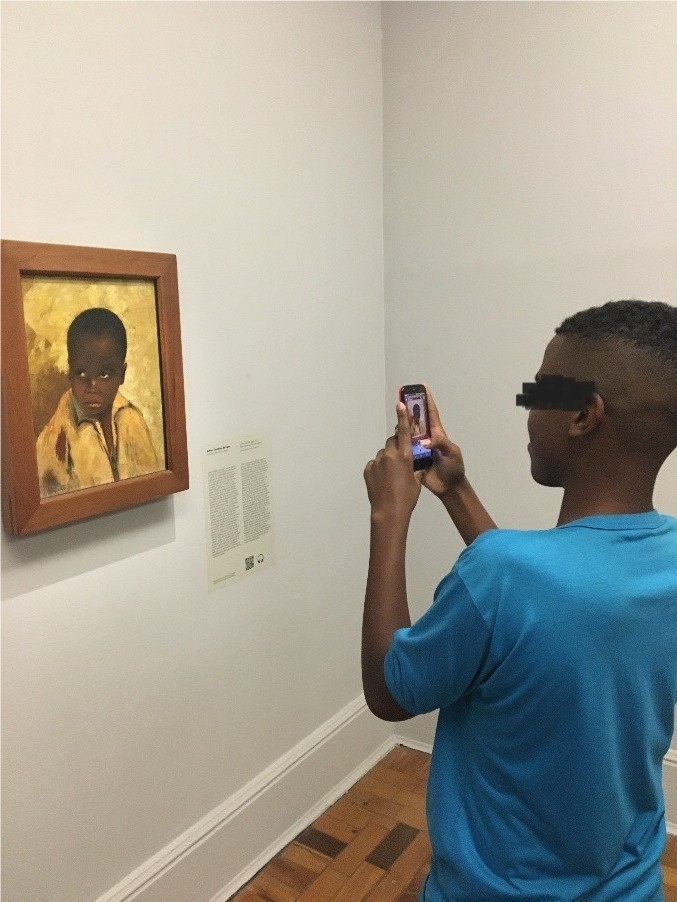
\includegraphics[width=\textwidth]{Imagem1.jpg}
 \caption{Atividades de apreciação.}
 \label{fig1}
 \end{minipage}%
 \qquad
 \begin{minipage}{0.45\textwidth}
 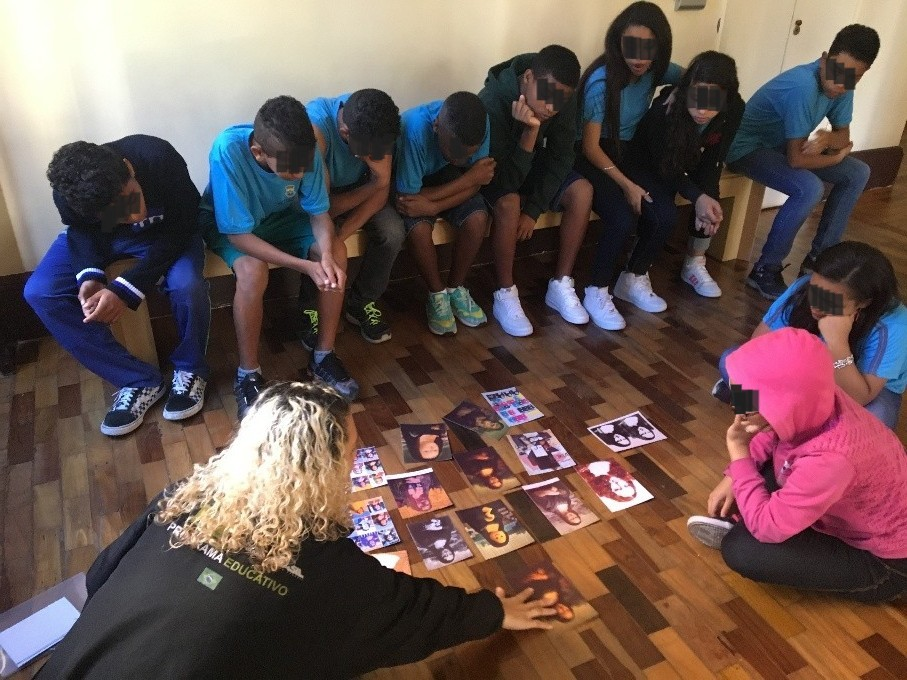
\includegraphics[width=\textwidth]{Imagem2.jpg}
 \caption{Adolescentes em atividades de apreciação.}
 \label{fig2}
 \end{minipage}%
 \source{Elaboração própria.} 
 \end{minipage}
\end{figure}

As Figuras \ref{fig1}, \ref{fig2}\footnote{As fotografias foram retiradas do arquivo pessoal da pesquisadora. Na época, sob orientação da Universidade Federal de Minas Gerais (UFMG), não foi necessário submeter o projeto ao comitê de ética, pois considerou-se que as imagens não expunham os educandos. Além disso, a pesquisadora tinha autorização para desenvolver o trabalho, já que a escola detinha os termos de autorização assinados no ato da matrícula dos alunos. Além disso, todas as imagens estão com alterações para evitar a identificação dos educandos.} apresentam alunos analisando obras de arte em grupo. Nessas atividades, as discussões foram bastante profícuas, pois promoveram engajamento de todos os participantes. Eles entenderam que as obras fazem parte de um contexto histórico e cultural. Essa percepção, de certo modo, dá subsídios para a crítica informada. Com isso, os estudantes relataram mais interesse pela arte, pelo desenvolvimento do escopo crítico, do domínio de alguns conceitos, o que lhes permitiu expressar suas opiniões de maneira mais articulada. Essa habilidade é importante, pois estimula a formação de um público mais consciente e culturalmente engajado \cite{hernandez2000educacao}.

\subsection{Contextualização}\label{sec-modelo}
O segundo eixo, a contextualização, integra a apreciação teórica à prática artística. Ao situar as obras em seus respectivos contextos histórico e cultural, os educadores ampliam a compreensão dos alunos sobre a arte e sua relevância social. Essa conexão é importante, já que a produção artística sempre reflete influências sociais, políticas e culturais de seu tempo. Conforme pontuam \textcite{lopes2013metodologias}, “compreender a obra de arte implica conhecer o contexto que a gerou”.

As Figuras \ref{fig3}, \ref{fig4}, \ref{fig5}, \ref{fig6}, extraídas do capítulo “Arte e Espaços urbanos” do livro didático Teláris Arte, exemplificam a aplicação dessa metodologia ao relacionar períodos artísticos com seus contextos socioculturais. A análise do material demonstrou que as discussões contextualizadas auxiliam no desenvolvimento e estimulam a criação de oportunidades para o entendimento e a apreciação de diversas narrativas culturais expressas na arte \cite{barbosa2010arte}.

\begin{figure}[h!]
 \centering
 \begin{minipage}{.9\textwidth}
 \begin{minipage}{.45\textwidth}
 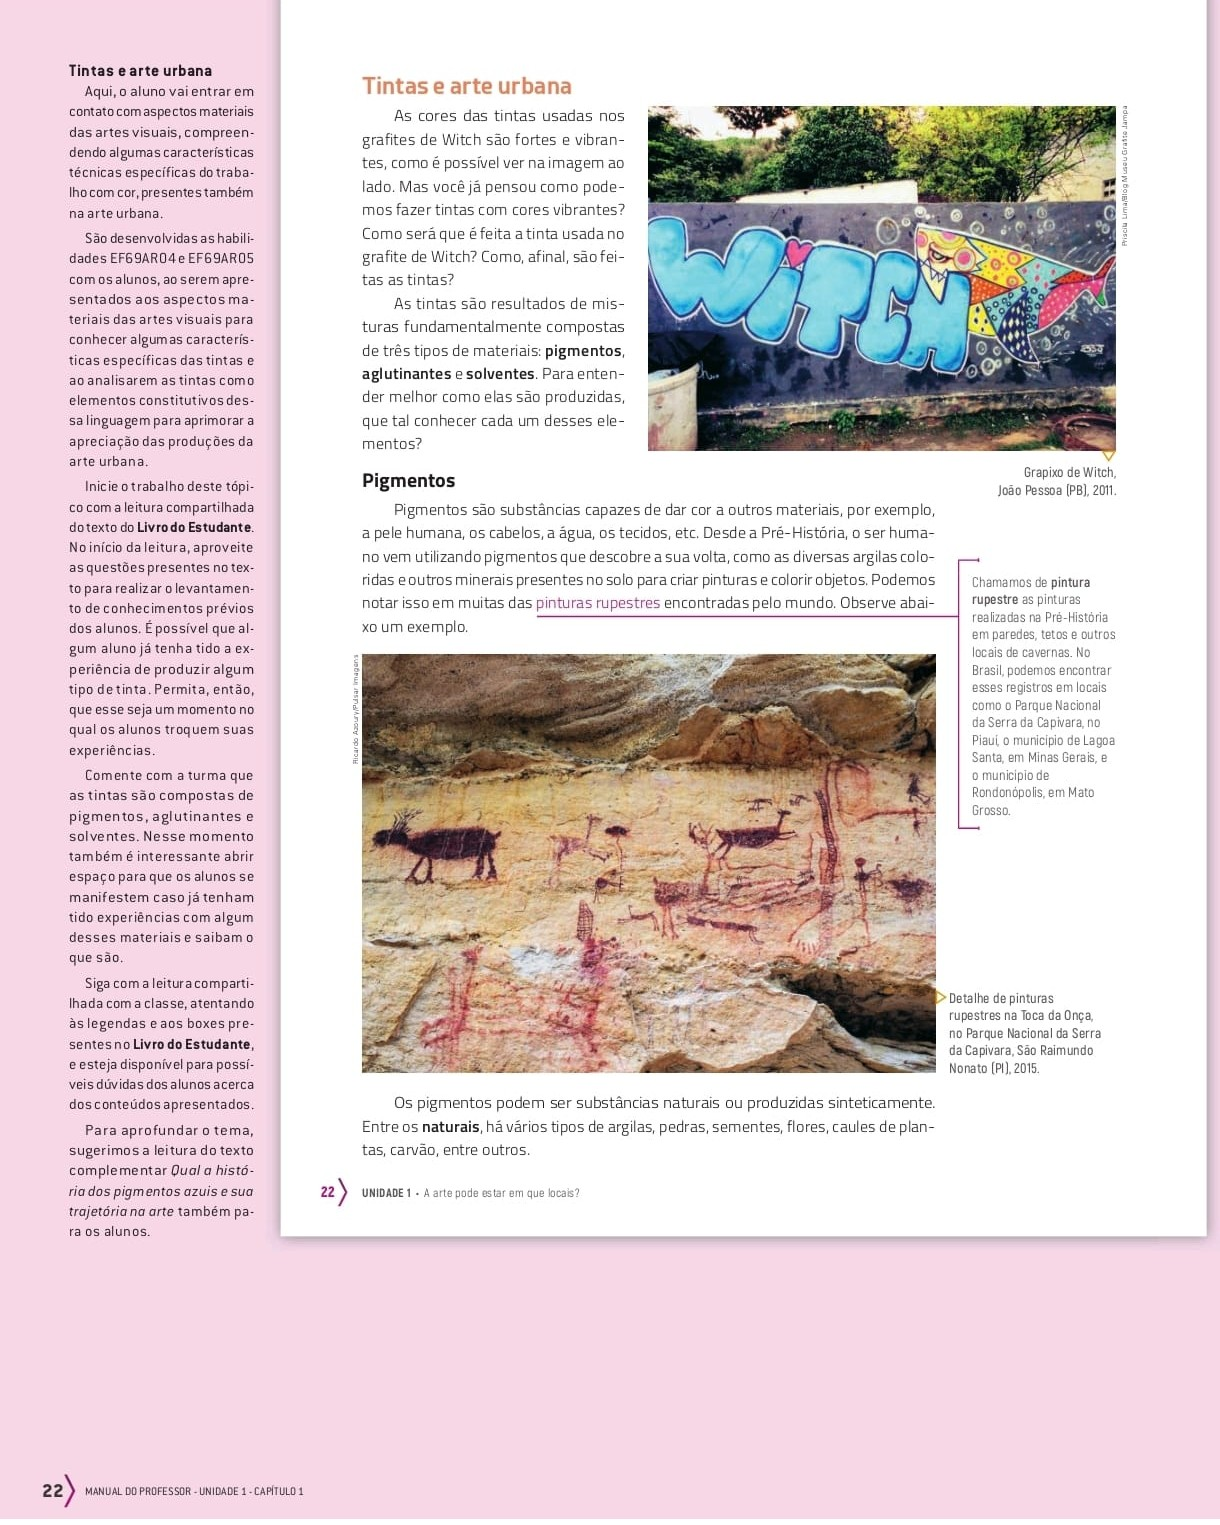
\includegraphics[width=\textwidth]{Imagem3.jpeg}
 \caption{Períodos artísticos com seus contextos socioculturais.}
 \label{fig3}
 \end{minipage}%
 \qquad
 \begin{minipage}{0.45\textwidth}
 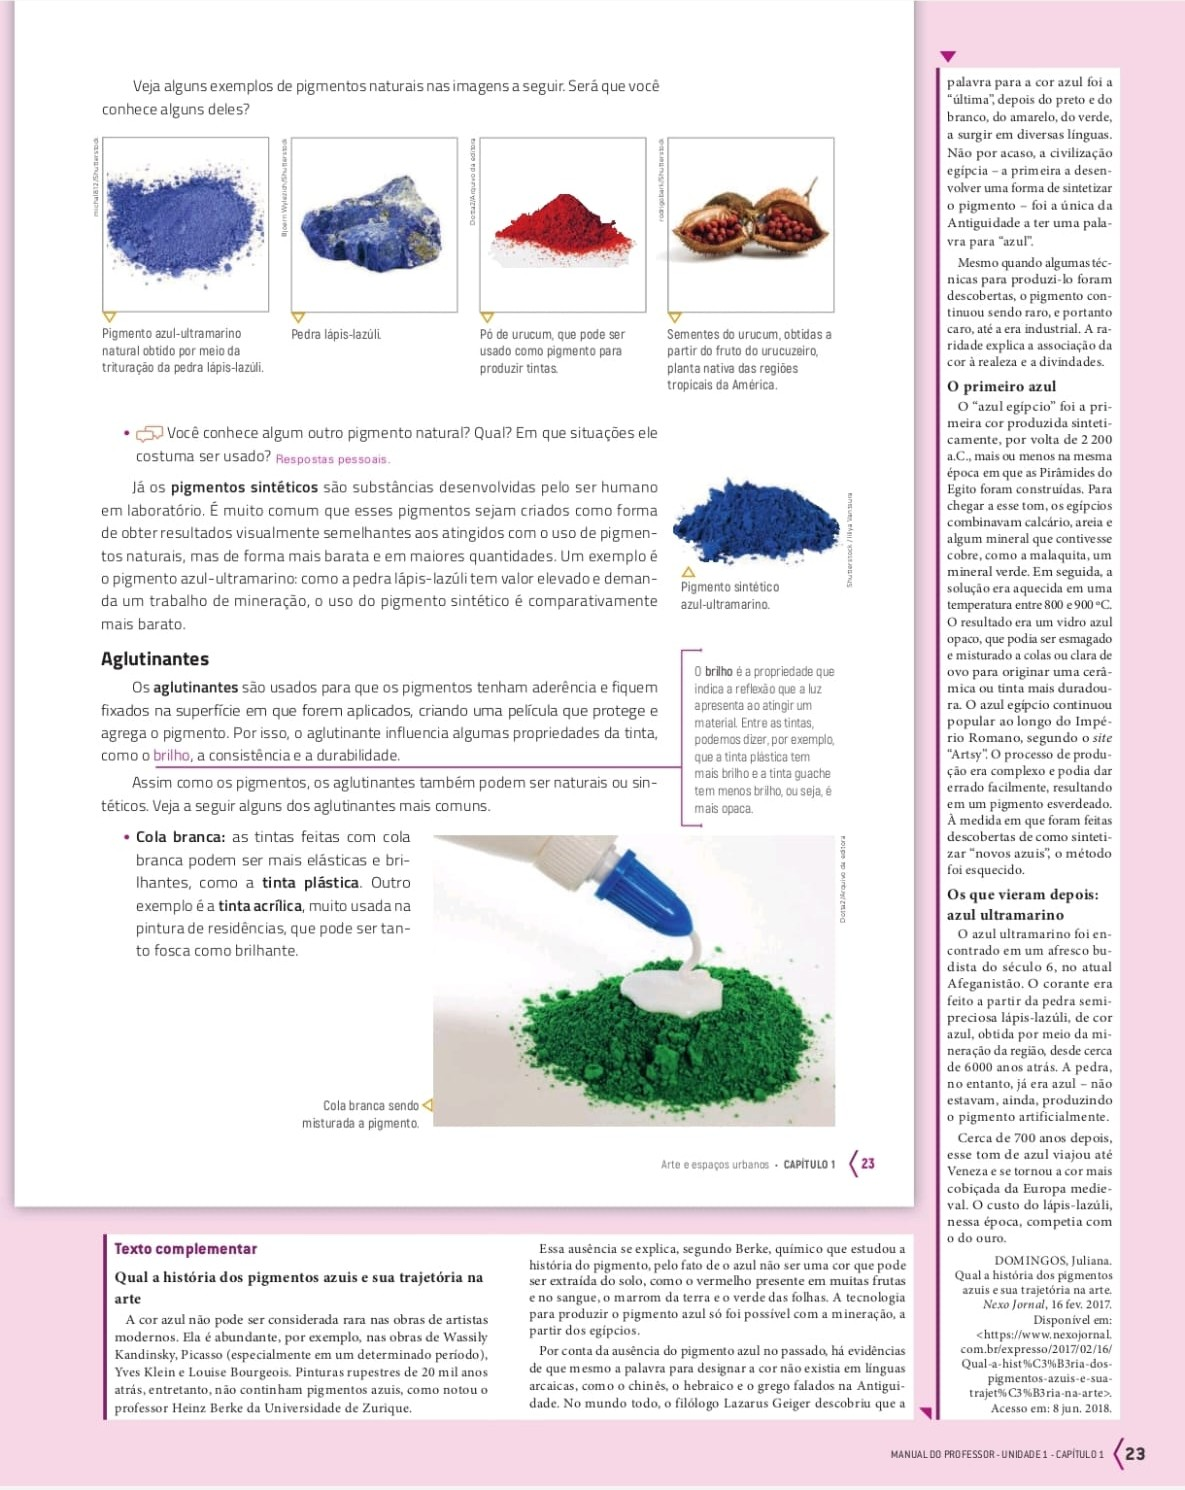
\includegraphics[width=\textwidth]{Imagem4.jpeg}
 \caption{Períodos artísticos com seus contextos socioculturais.}
 \label{fig4}
 \end{minipage}%
 \source{\cite[p. 22-23]{pougy2018teleris}.} 
 \end{minipage}
\end{figure}

\begin{figure}[h!]
 \centering
 \begin{minipage}{.9\textwidth}
 \begin{minipage}{.45\textwidth}
 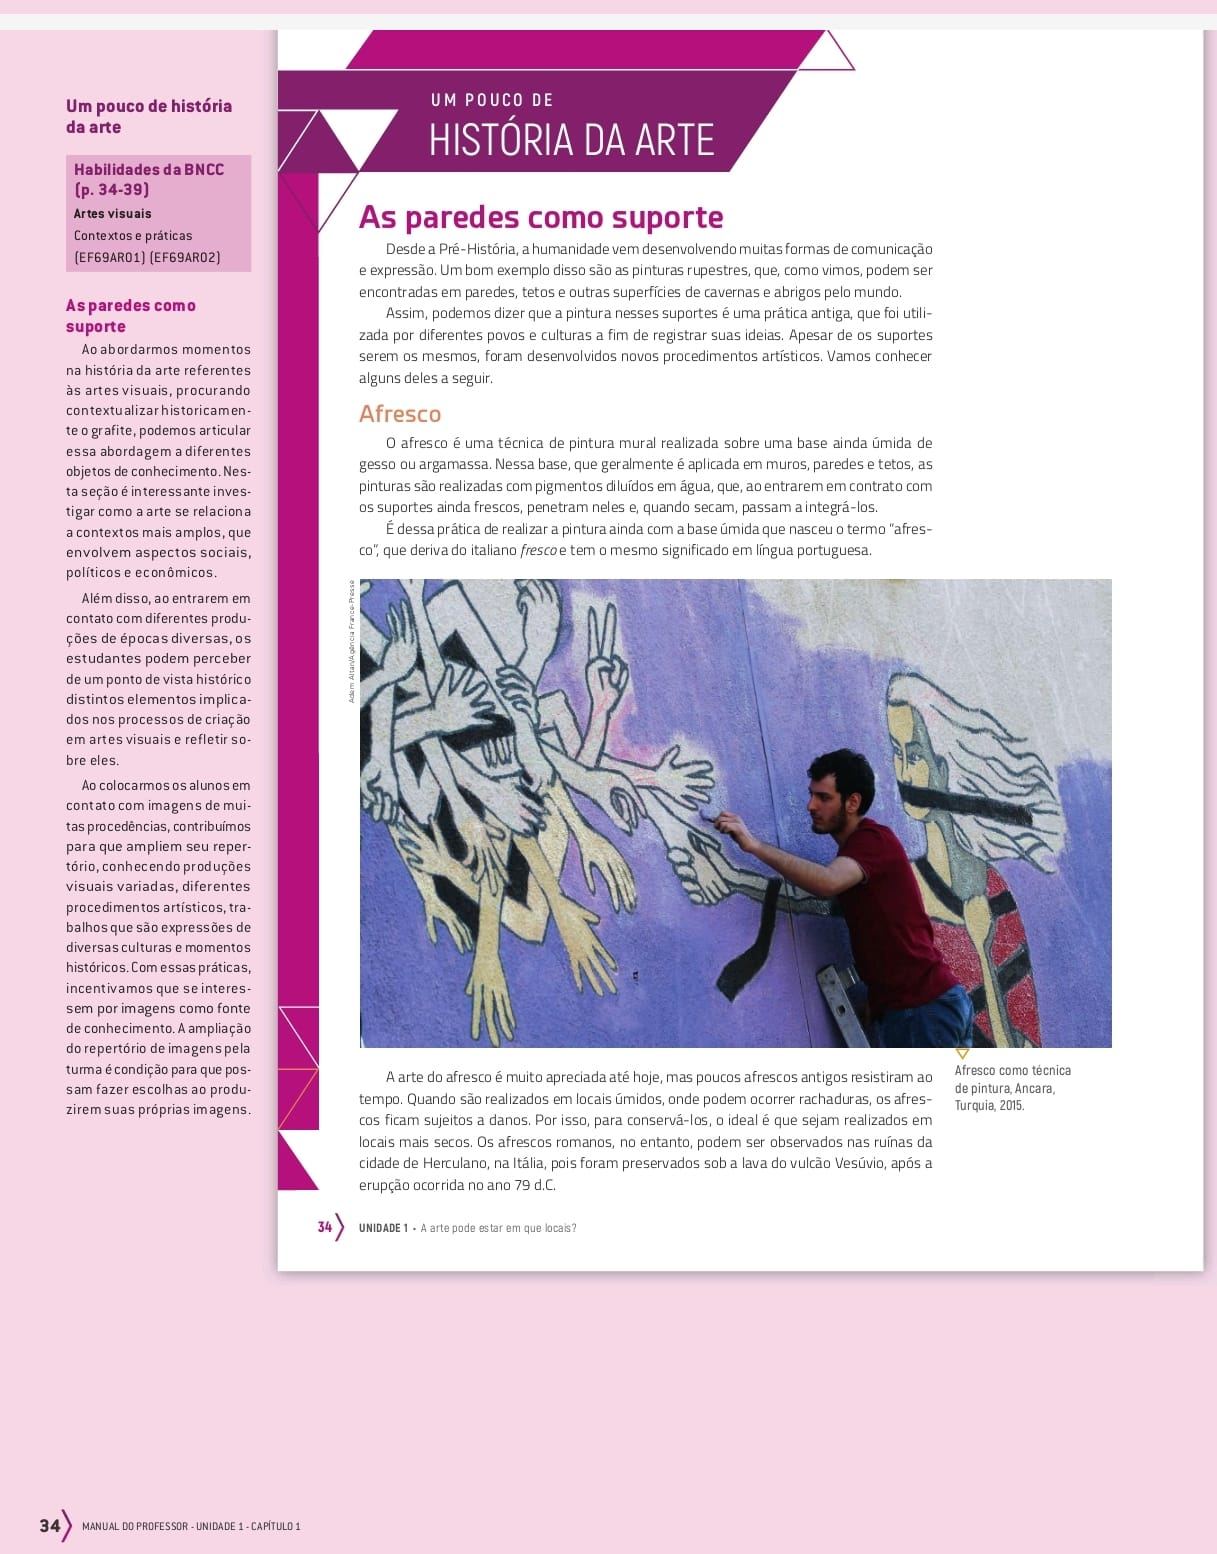
\includegraphics[width=\textwidth]{Imagem5.jpeg}
 \caption{Períodos artísticos com seus contextos socioculturais.}
 \label{fig5}
 \end{minipage}%
 \qquad
 \begin{minipage}{0.45\textwidth}
 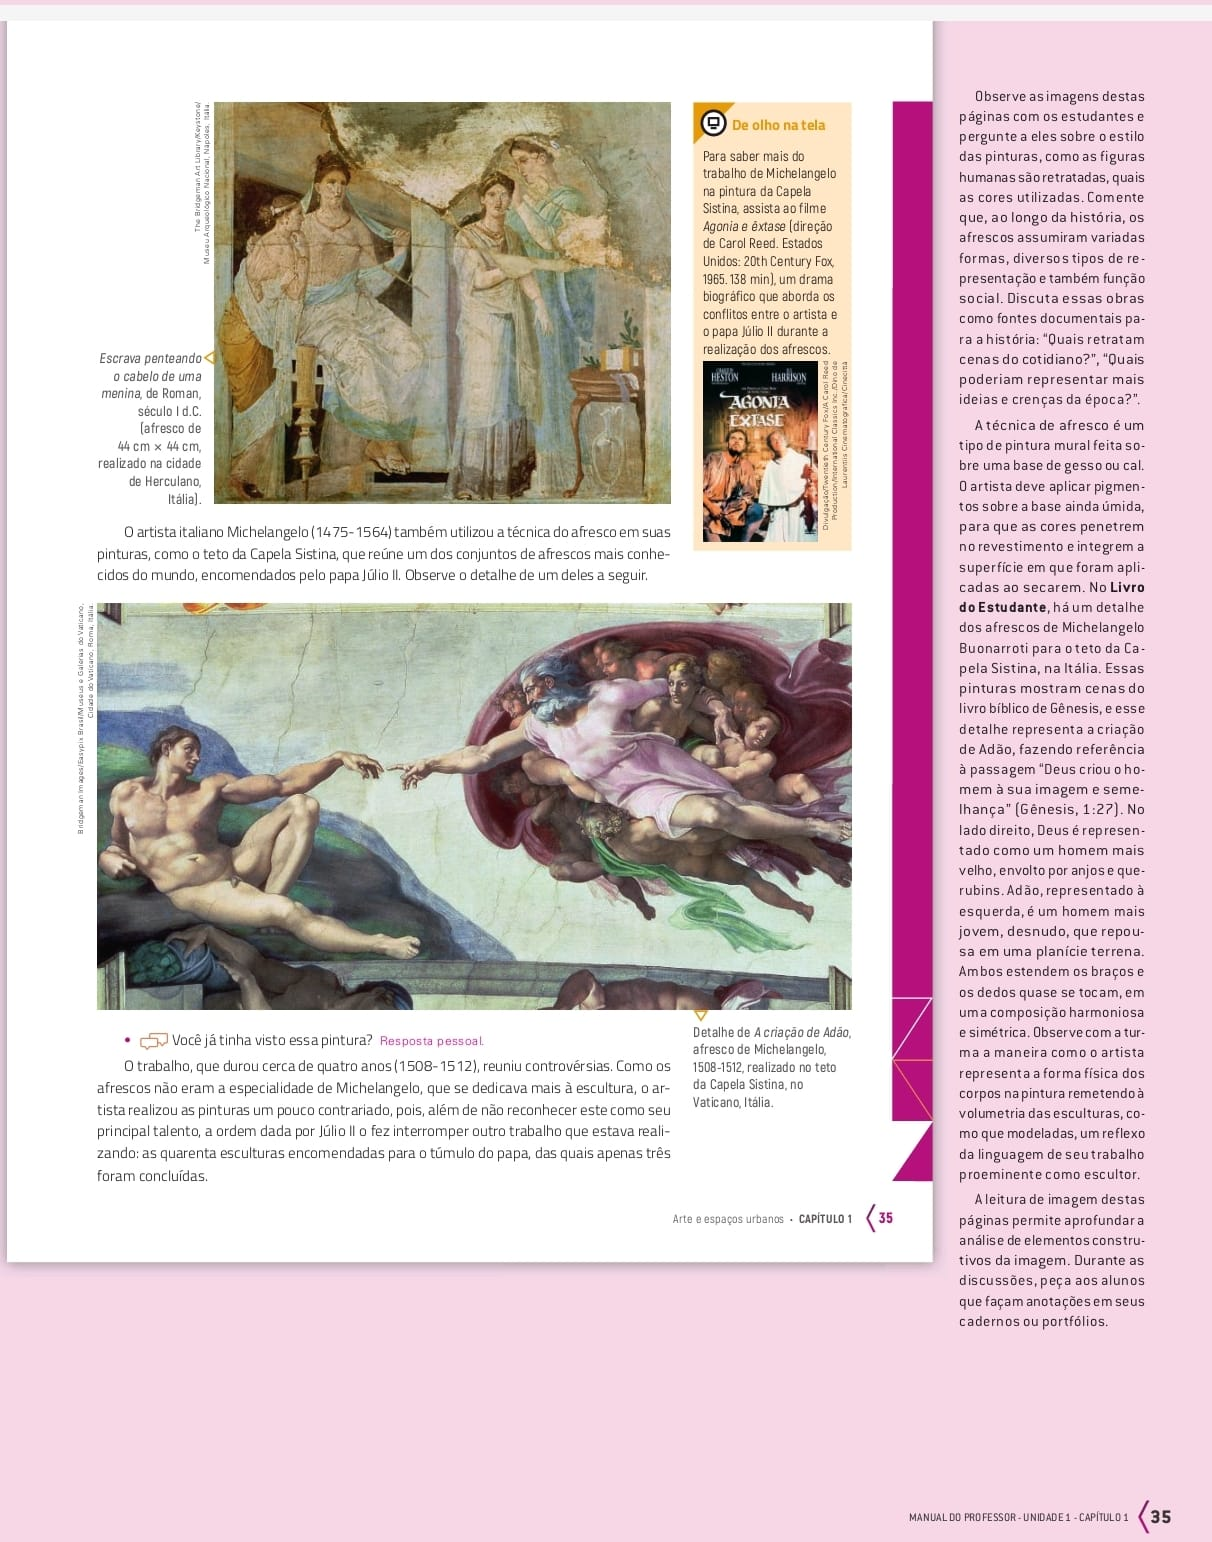
\includegraphics[width=\textwidth]{Imagem6.jpeg}
 \caption{Períodos artísticos com seus contextos socioculturais.}
 \label{fig6}
 \end{minipage}%
 \source{\cite[p. 24-25]{pougy2018teleris}.} 
 \end{minipage}
\end{figure}

%\begin{figure}[h!]
%    \centering
%    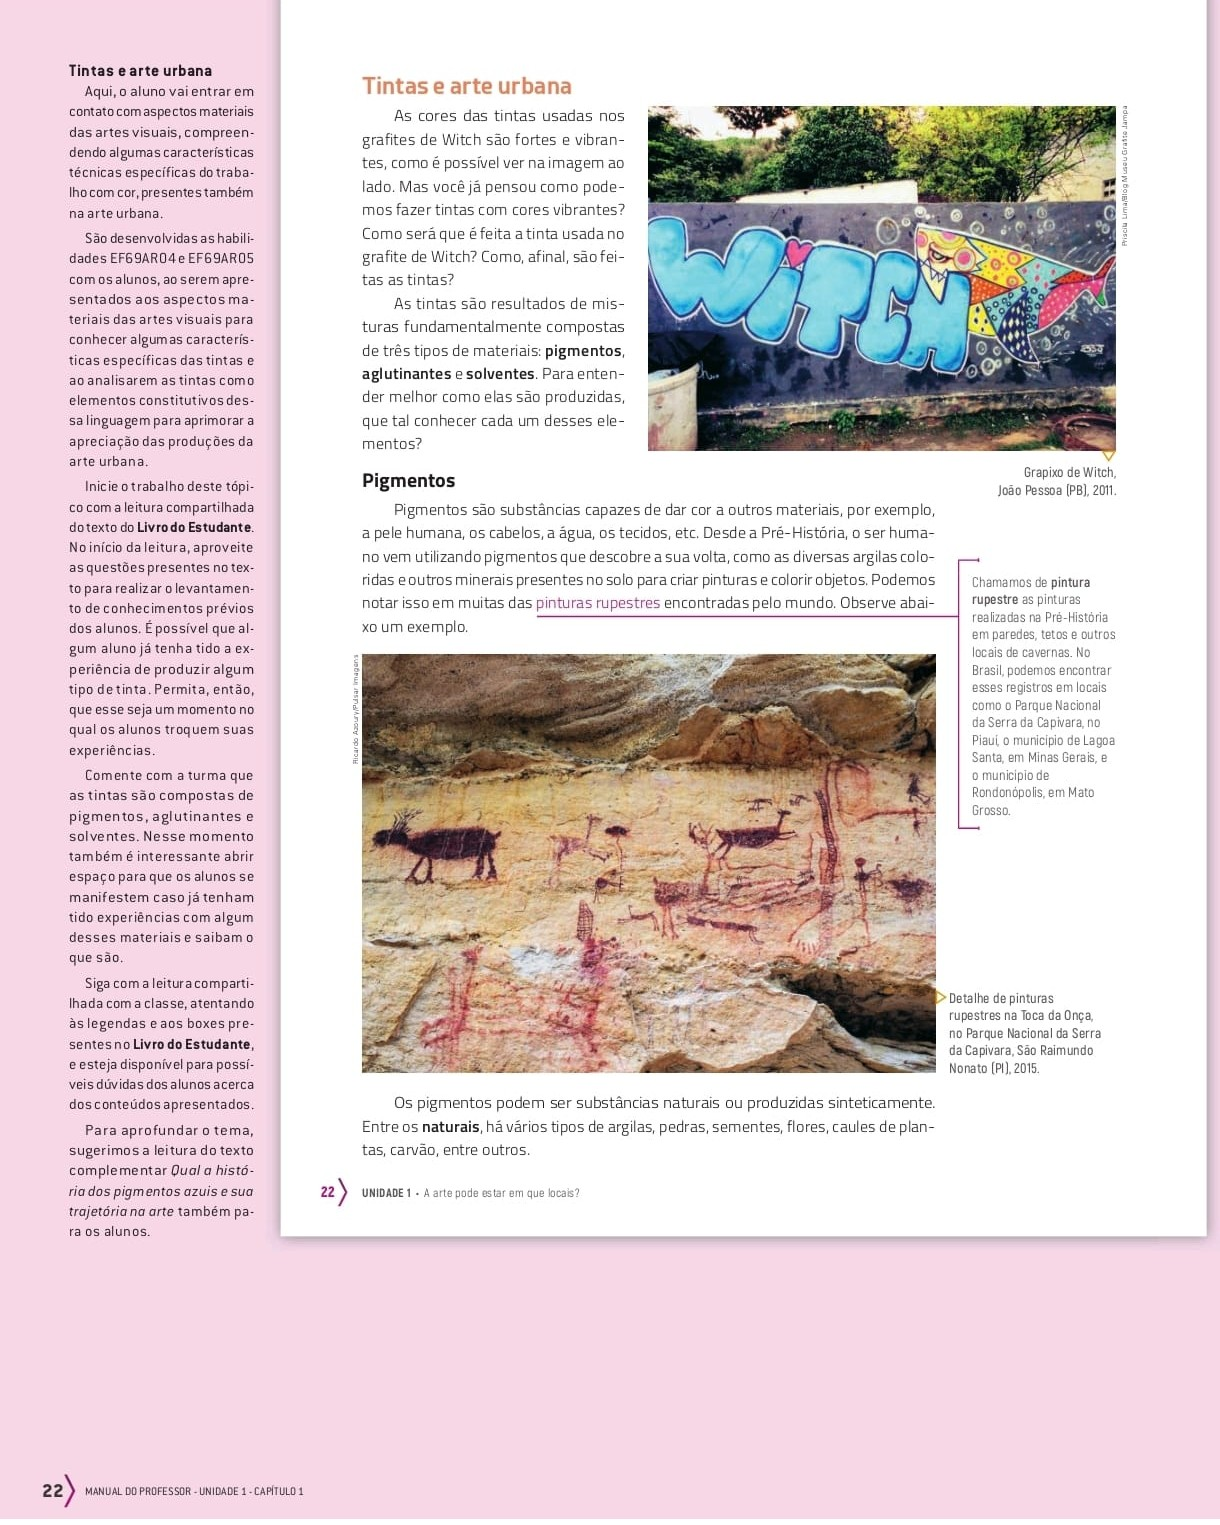
\includegraphics[width=0.75\linewidth]{Imagem3.jpeg}
%    \caption{Períodos artísticos com seus contextos socioculturais.}
%    \label{fig3}
%    \source{Pougy; Vilela, 2018b, p. 22}
%\end{figure}

%\begin{figure}[h!]
%    \centering
%    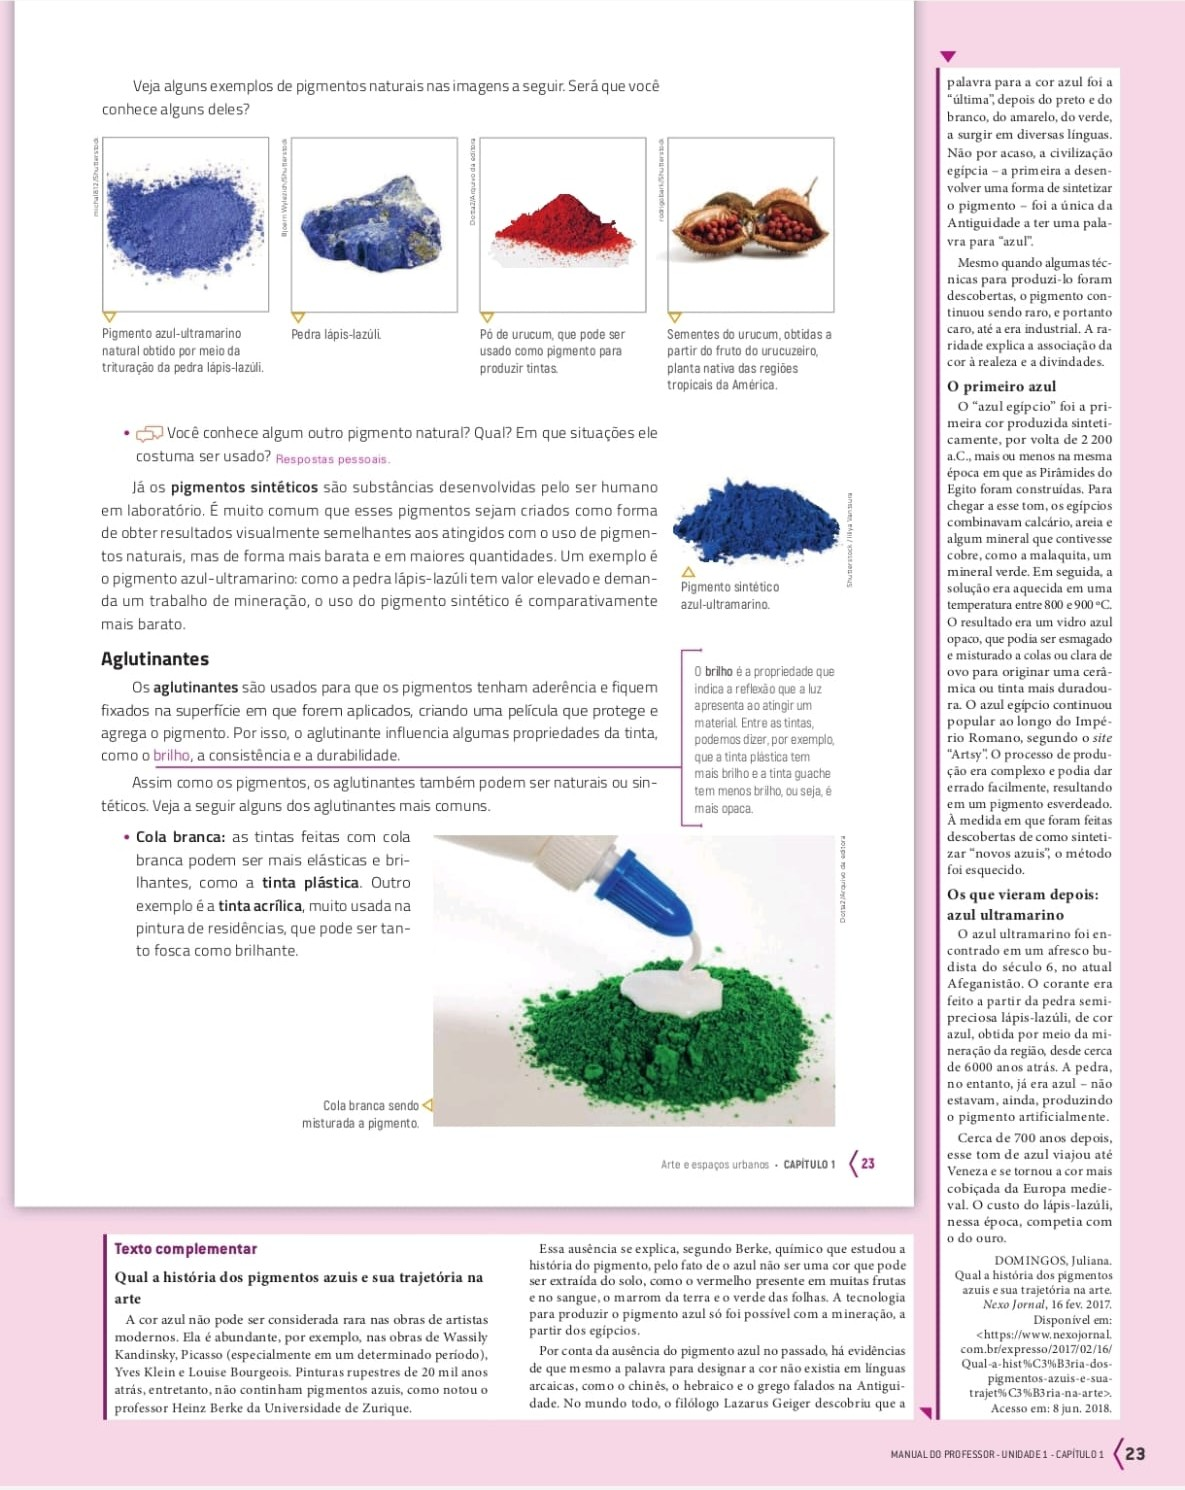
\includegraphics[width=0.75\linewidth]{Imagem4.jpeg}
%    \caption{Períodos artísticos com seus contextos socioculturais.}
%    \label{fig4}
%    \source{Pougy; Vilela, 2018b, p. 23}
%\end{figure}

%\begin{figure}[h!]
%    \centering
%    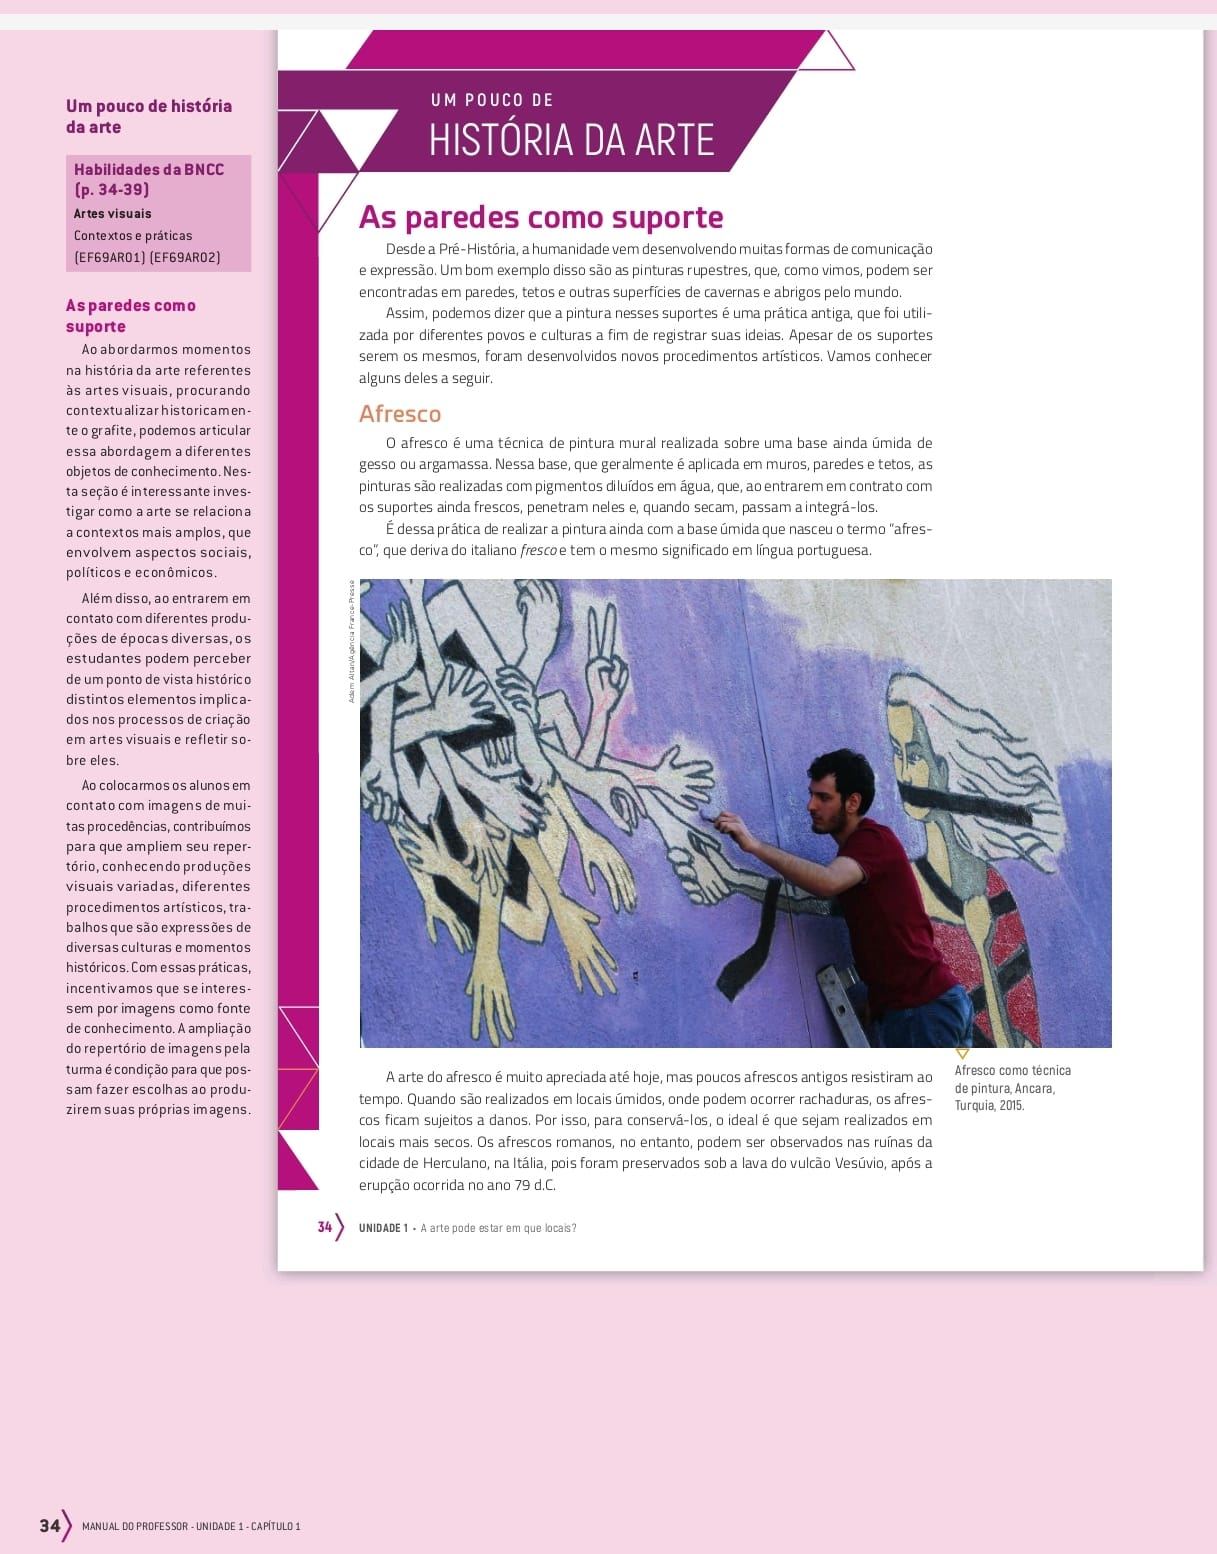
\includegraphics[width=0.75\linewidth]{Imagem5.jpeg}
%    \caption{Períodos artísticos com seus contextos socioculturais.}
%    \label{fig5}
%    \source{Pougy; Vilela, 2018b, p. 22}
%\end{figure}

%\begin{figure}[h!]
%    \centering
%    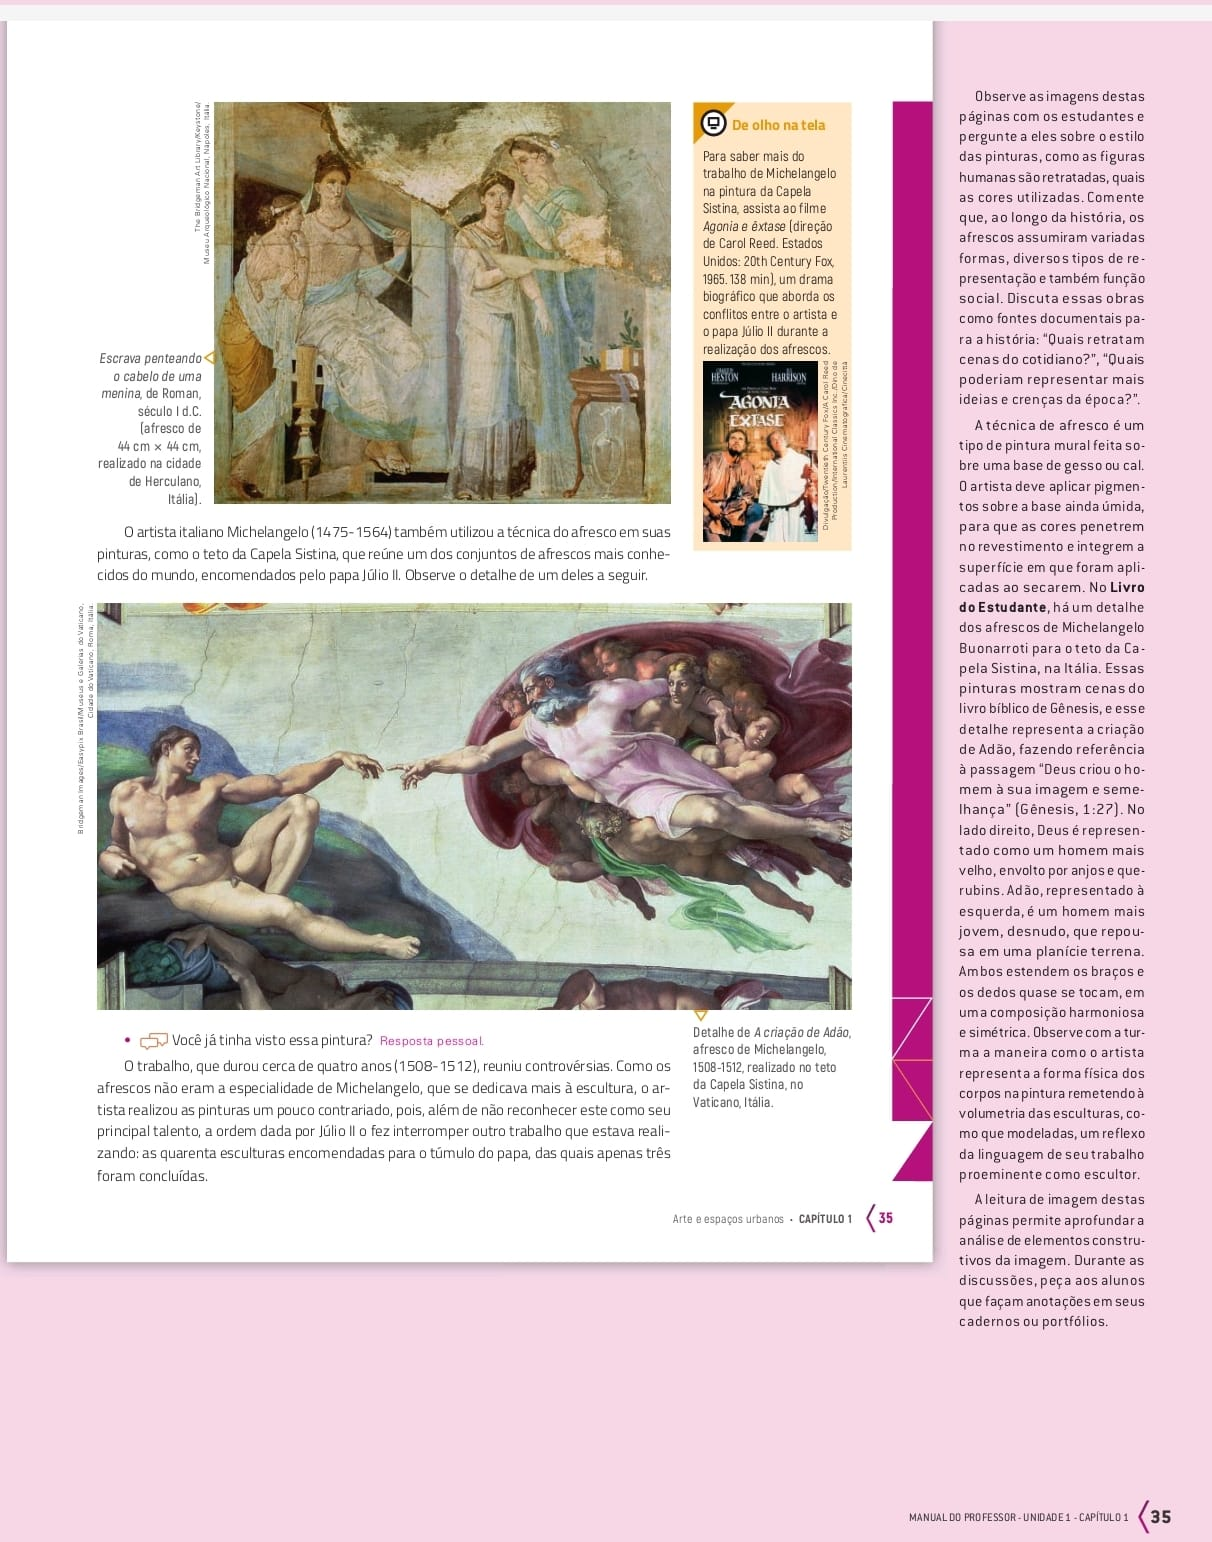
\includegraphics[width=0.75\linewidth]{Imagem6.jpeg}
%    \caption{Períodos artísticos com seus contextos socioculturais.}
%    \label{fig6}
%    \source{Pougy; Vilela, 2018b, p. 23}
%\end{figure}

A coleção Teláris Arte (livro didático presente no Plano Nacional do Livro Didático – PNLD) apresenta conexões com a Abordagem Triangular, presentes nas atividades e orientações ao professor. A primeira atividade da Unidade 1 (Introdução) desenvolve-se a partir da práxis artística e finda com reflexões artísticas. Explora-se o tema “Grafite” em diversas vertentes, intercruzando saberes referentes à Cultura Visual, produzindo a transdisciplinaridade, isto é, promovendo conexões tanto no contexto escolar quanto fora dele, com questões sociais pertinentes à formação cidadã, pela qual também preza a BNCC.

\subsection{Criação}\label{sec-organizacao}
O eixo de criação, por sua vez, destaca-se como um espaço para a expressão pessoal e a aplicação das habilidades adquiridas nos dois eixos anteriores. A prática da criação artística provoca a experimentação de técnicas e estilos e incentiva a autoexpressão e a exploração de temas significativos no contexto da escola. Desse modo, os educandos que se envolvem em projetos de criação mostram-se mais autoconfiantes para expressarem-se artisticamente.

As Figuras \ref{fig7}, \ref{fig8}, \ref{fig9} exibem uma galeria de trabalhos criativos dos alunos. Durante a prática de criar, logo depois da apreciação e da contextualização, proporcionou-se um ambiente rico para a experimentação e para a inovação. Os alunos foram incentivados a explorar sua identidade por meio da arte; criaram obras que refletiam suas vivências e visões de mundo.

\begin{figure}[h!]
 \centering
 \begin{minipage}{.9\textwidth}
 \begin{minipage}{.45\textwidth}
 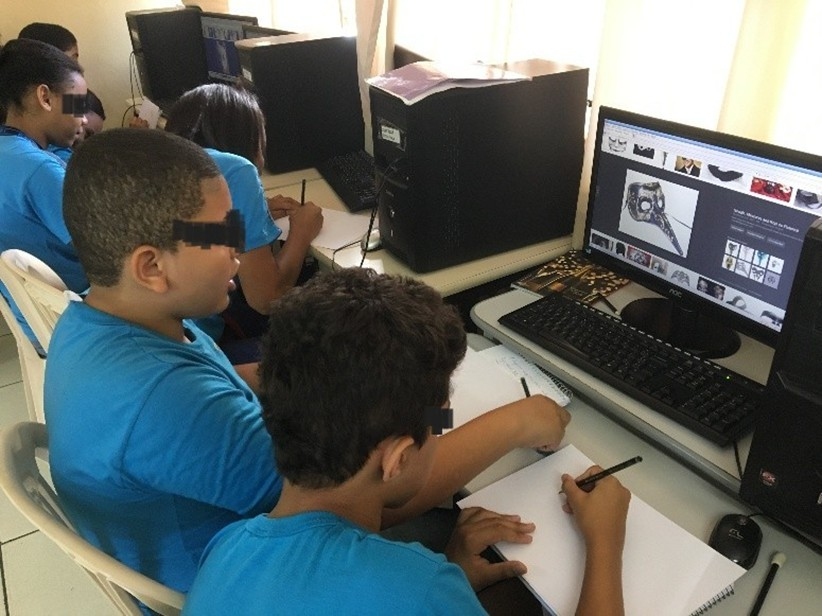
\includegraphics[width=\textwidth]{Imagem7.jpg}
 \caption{Trabalhos de alunos durante o projeto educativo.}
 \label{fig7}
 \end{minipage}%
 \qquad
 \begin{minipage}{0.45\textwidth}
 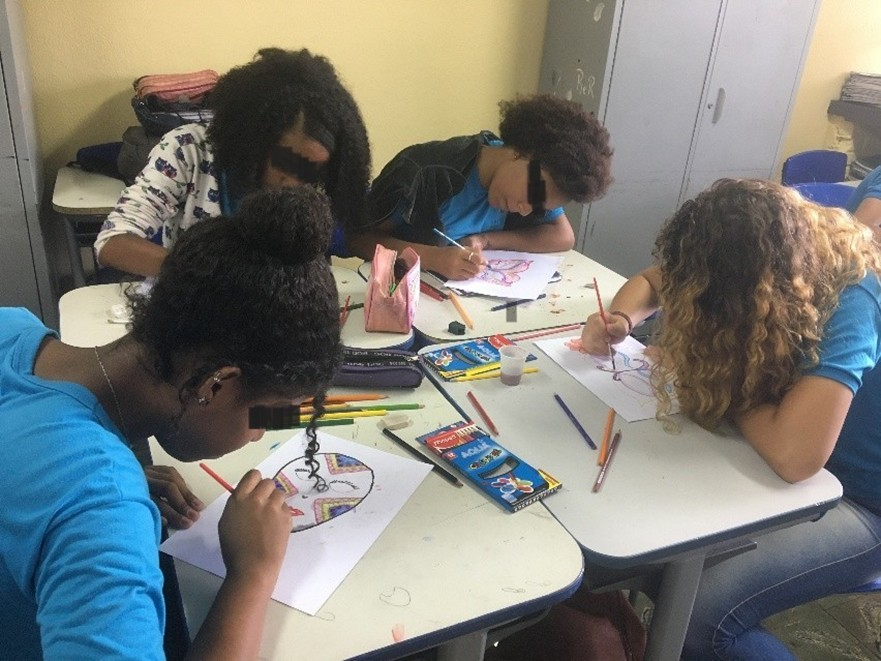
\includegraphics[width=\textwidth]{Imagem8.jpg}
 \caption{Trabalhos de alunos durante o projeto educativo.}
 \label{fig8}
 \end{minipage}%
 \source{Elaboração própria.}
 \end{minipage}
\end{figure}

\begin{figure}[h!]
    \centering
    \begin{minipage}{.55\textwidth}
    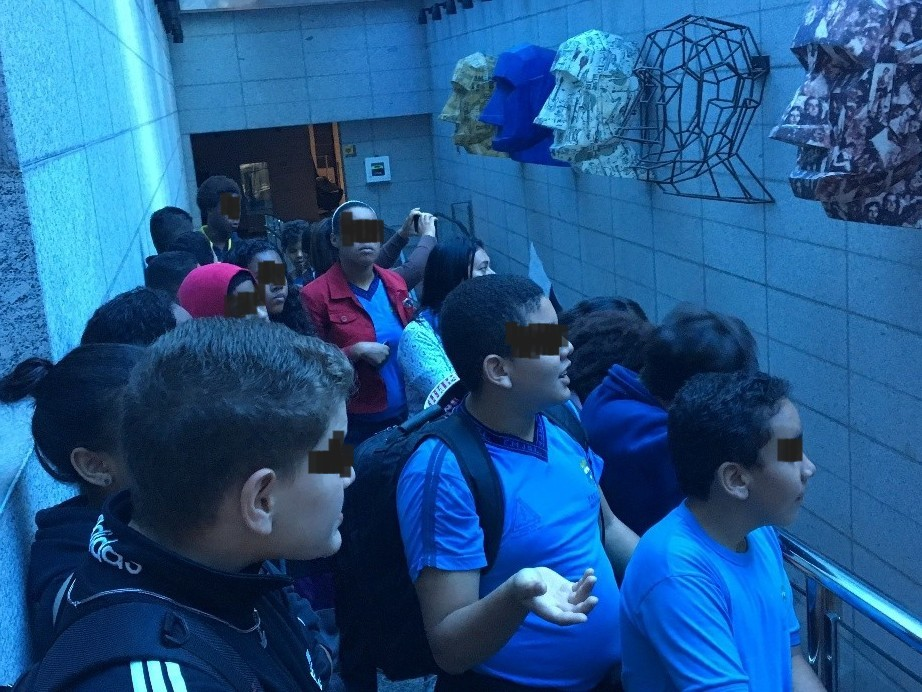
\includegraphics[width=\linewidth]{Imagem9.jpg}
    \caption{Trabalhos de alunos durante o projeto educativo.}
    \label{fig9}
    \source{Elaboração própria.}
    \end{minipage}
\end{figure}

Durante a criação artística, notamos que os resultados eram singulares para cada sujeito. Entendemos que isso não poderia ser diferente, pois cada indivíduo tem um arcabouço cultural, cada um tem alguma habilidade específica, as quais se desenvolvem a partir de suas bagagens históricas e pessoais, influenciando diretamente o processo de aprendizagem. De certa maneira, podemos evidenciar como essas subjetividades se entrelaçam e se conectam a outras histórias compartilhadas durante as aulas.

Como ressaltado por \textcite{minayo2010pesquisa}, a criação artística em ambientes educacionais promove mais que o desenvolvimento de habilidades técnicas. Todo o processo de se aplicar uma metodologia visa à formação do pensamento crítico que, por sua vez, questiona e reinterpreta a realidade. Os dados coletados indicam que a abordagem triangular fomenta um ciclo virtuoso de aprendizado: a apreciação instiga a curiosidade, a contextualização oferece entendimento mais aprofundado e a criação permite que os alunos expressem suas próprias visões e experiências, suas subjetividades, seus traços identitários. É importante ressaltar que a tecnologia possibilitou criar formas de expressão, além de ampliar o alcance e a visibilidade do trabalho dos alunos, conectando-os a um público mais amplo.

\section{Resultados}\label{sec-organizacao-latex}
Em suma, os resultados obtidos a partir da aplicação da abordagem triangular demonstram sua eficácia na promoção da educação artística mais integrada ao contexto sociocultural. Os eixos não operam isoladamente, mas interagem com o objetivo de construir uma experiência educacional integrada, dando oportunidades aos alunos de se tornarem críticos, criativos e mais conectados com o contexto da arte.

Além disso, a combinação dos três eixos mostrou-se eficaz em desenvolver a capacidade de resolução de problemas, uma competência essencial no século 21. Ao integrar a apreciação crítica, a contextualização histórica e a prática criativa, os alunos ampliaram seu conhecimento sobre arte e aprenderam a aplicar esse conhecimento em situações da vida real. Com método e aplicação, realizaram a arte de fruir abstrações \cite{minayo2010pesquisa,bourdieu1996distincao,dewey1934art}.

Outro ponto relevante observado foi a influência da abordagem triangular na formação de uma comunidade de aprendizagem na sala de aula. Os alunos, ao discutirem suas interpretações e criações, cultivaram um ambiente colaborativo que favoreceu a troca de ideias e o respeito pelas diferentes perspectivas. Essa dinâmica de sala de aula foi vista como exemplo a ser seguido, fortaleceu a empatia e o engajamento entre os alunos.

Os resultados positivos da aplicação da abordagem reforçam sua adoção e difusão. Essa metodologia deve, pois, ser incentivada e divulgada em espaços educacionais, com formação contínua para os educadores a fim de garantir que a abordagem triangular seja aplicada de maneira eficaz e contextualizada, de modo a atender às necessidades e realidades dos alunos.

\section{Considerações finais}\label{sec-titulo}
A implementação da abordagem triangular no ensino de arte se mostra um caminho promissor para a formação de alunos mais críticos, criativos e conscientes de seu papel na sociedade. Ao integrar seus eixos de formação, essa abordagem pode fomentar a compreensão mais profunda da arte e de sua relevância cultural, colocando os alunos como protagonistas ativos na construção de seu conhecimento.

Conforme enfatizado por \textcite{barbosa2018debate}, a abordagem visa promover espaços de reflexão, onde os alunos aprendem a articular suas opiniões e a respeitar diferentes pontos de vista. Além disso, a arte pode ser compreendida dentro de um quadro histórico e cultural mais amplo. Como destacado por \textcite{lopes2013metodologias}, essa conexão entre passado e presente possibilita que os estudantes vejam a arte como uma expressão estética e como um reflexo das lutas, valores e transformações sociais.

O eixo de criação, por sua vez, torna-se uma porta de entrada para a autoexpressão e a exploração da identidade. A prática criativa encoraja os alunos a experimentar, arriscar e desenvolver suas habilidades, tanto técnicas quanto intuitivas \cite{minayo2010pesquisa}. O espaço de liberdade criativa, como foi observado, ofereceu oportunidades para que os alunos construíssem uma relação pessoal com a arte, uma intimidade e aprofundamento com os seus próprios valores e crenças.

Ademais, a abordagem triangular não deve ser vista como uma receita metodológica única, mas como um convite à reflexão e à adaptação. De certa maneira, um convite a colocar em prática o que preza a BNCC. E cada educador, ao implementar essa metodologia, deve considerar o contexto de sua sala de aula e as necessidades específicas de seus alunos. A flexibilidade e a abertura para a inovação são características que podem fortalecer ainda mais a sua eficácia. A tecnologia pode facilitar o acesso às obras de arte e a sua consequente fruição. Vídeos e plataformas de discussão \textit{online} podem potencializar essa interação, permitindo que os alunos explorem diversas interpretações e contextos de maneira mais dinâmica, como preza a Competência 5 – Cultura digital – da BNCC.

Além das considerações já mencionadas, é importante ressaltar a necessidade de acompanhamento contínuo da aplicação da metodologia triangular. A formação inicial e continuada dos educadores é essencial para que eles se sintam seguros e preparados para integrar esses eixos em suas práticas pedagógicas. Investir em formações e em trocas de experiências entre professores pode enriquecer todo o processo e aprimorar outras práticas educativas.

Um ponto relevante a ser considerado é a avaliação de todo o processo, suas fases, seus eixos. A avaliação deve ir além da simples mensuração de habilidades técnicas, abrangendo também o desenvolvimento de competências socioemocionais e a capacidade crítica dos alunos. É, pois, necessário desenvolver instrumentos de avaliação que considerem esses aspectos, garantindo que a eficácia da abordagem triangular seja devidamente mensurada e aprimorada.

Este estudo conclui, portanto, que a abordagem triangular é um recurso pedagógico relevante que pode auxiliar o ensino de arte. A formação integral promovida por essa metodologia prepara os alunos para uma compreensão mais sensível da arte e da cultura, contribuindo para a formação de indivíduos capazes de pensar criticamente e agir de maneira ética em sua sociedade. O desafio agora é promover a adoção e a pesquisa contínua sobre essa abordagem, visando sempre a melhoria da prática educativa e o fortalecimento do papel da arte na educação.

As experiências relatadas nesta pesquisa indicam que a adoção dessa abordagem melhora a relação dos alunos com a arte e também os empodera. A incorporação de tecnologias digitais, como recursos multimídia e de pesquisa \textit{online}, enriquece essa contextualização, tornando-a mais acessível e interativa. O educador torna-se um agente mediador e facilitador, aquele que oportuniza a produção de conhecimento. Acreditamos que a implementação dessa abordagem em larga escala pode contribuir para uma transformação no ensino de arte. O desafio agora é promover a adoção e a pesquisa contínua sobre a abordagem triangular, visando sempre a melhoria da prática educacional e o fortalecimento do papel da arte na educação, especialmente com a integração da tecnologia como um aliado nesse processo. Na visão freiriana, é colocar em prática um modelo de educação para transformar as mentes que vão transformar o mundo.

\printbibliography\label{sec-bib}
% if the text is not in Portuguese, it might be necessary to use the code below instead to print the correct ABNT abbreviations [s.n.], [s.l.]
%\begin{portuguese}
%\printbibliography[title={Bibliography}]
%\end{portuguese}


%full list: conceptualization,datacuration,formalanalysis,funding,investigation,methodology,projadm,resources,software,supervision,validation,visualization,writing,review
\begin{contributors}[sec-contributors]
\authorcontribution{Laura Paola Ferreira}[conceptualization,investigation,methodology,writing,review]
\authorcontribution{Danilo Rodrigues Zinatelli César}[conceptualization,investigation,methodology,writing,review]
\authorcontribution{Eloiza Mara de Paula Rossoni}
[writing,review]
\end{contributors}

\begin{dataavailability}
\txtdataavailability{datanotav} % options: dataavailable, dataonly, databody, datanotav, nodata
\end{dataavailability}

\end{document}